\documentclass[11pt,a4paper]{article}
\usepackage[T1]{fontenc}
\usepackage[utf8]{inputenc}
\usepackage{lmodern}
\usepackage{microtype}
\usepackage[a4paper,margin=28mm]{geometry}
\usepackage[numbers,sort&compress]{natbib}
\usepackage{amsmath,amssymb,amsthm}
\usepackage{booktabs}
\usepackage{graphicx}
\usepackage[font=small,labelfont=bf]{caption}
\usepackage{algorithm}
\usepackage{algpseudocode}
\usepackage{xcolor}
\usepackage{hyperref}
\usepackage[nameinlink,noabbrev]{cleveref}
\hypersetup{colorlinks=true,linkcolor={blue!50!black},citecolor={blue!50!black},urlcolor={blue!50!black}}
\captionsetup[figure]{name=Fig.}
\graphicspath{{../results/figures/}}
\newtheorem{proposition}{Proposition}[section]
\newtheorem{lemma}[proposition]{Lemma}
\newcommand{\E}{\mathbb{E}}
\newcommand{\Var}{\operatorname{Var}}
\newcommand{\Cov}{\operatorname{Cov}}
\newcommand{\Corr}{\operatorname{Corr}}
\crefname{lemma}{Lemma}{Lemmas}

\title{Parallel Monte Carlo and Finite-Difference Pricing\\ in the Black--Scholes Model with MPI}
\author{Xiangyu Luo\thanks{Southwest Petroleum University, Chengdu, China (\href{mailto:louang.620@gmail.com}{louang.620@gmail.com}). Course project in Large-Scale Scientific Computing Infrastructure, 2024.}}
\date{}

\begin{document}
\maketitle

\begin{abstract}
We study the parallel Monte Carlo pricing of European and discretely monitored arithmetic-average Asian call options in the Black--Scholes model and validate it against closed-form prices and a Crank--Nicolson finite-difference solver.
The pricer distributes independent random streams over MPI processes and merges the per-process results through eleven additive sufficient statistics, so that the parallel estimate, the control-variate coefficient and the standard error coincide with those of a single process for any division of the work; antithetic sampling and control variates are built into the same statistics.
We derive the variance of the antithetic and control-variate estimators in terms of correlations that are measured directly, and the predicted variance-reduction factors agree with those observed over independent replications to within one percent: with $2.56\times10^5$ paths the combination of both techniques reduces the variance of the European estimator by a factor of 27, and the geometric-Asian control variate reduces that of the Asian estimator by a factor of about 500.
The Crank--Nicolson solver with Rannacher start-up converges at second order in both time and space and matches the analytical European price to within $4\times10^{-5}$ for maturities of one to four years; without the start-up procedure, the price is equally accurate but the gamma at the strike is wrong by more than half of its value on the same grid, in quantitative agreement with a frozen-coefficient estimate of the damping of the payoff kink.
On a ten-core laptop with four performance and six efficiency cores, the pricer reaches a $3.5\times$ speed-up on 8 processes (efficiency 44\%).
A simple performance model shows that the strong-scaling speed-up is predicted by the weak-scaling efficiency, so that the loss of efficiency is a property of the shared hardware rather than of the parallel algorithm, which communicates a single gather of 213 bytes per process.
\end{abstract}

\noindent\textbf{Key words.} option pricing, Monte Carlo methods, variance reduction, Crank--Nicolson method, Rannacher time stepping, MPI, parallel scaling

\smallskip
\noindent\textbf{MSC codes.} 65C05, 65M06, 65M12, 91G60, 68W10

%% ==================================================================
\section{Introduction}\label{sec:intro}

Black and Scholes \citep{black1973} expressed the price of a European option on a stock following geometric Brownian motion (GBM) as the solution of a parabolic partial differential equation, and by the Feynman--Kac formula the same price is the discounted expectation of the payoff under the risk-neutral measure.
This duality between a differential equation and an expectation leads to the two families of numerical methods that dominate computational finance.
Deterministic grid methods discretise the PDE, and in one space dimension the Crank--Nicolson (CN) scheme \citep{crank1947} is fast, unconditionally stable and second-order accurate \citep{duffy2006,wilmott1995}.
The non-smooth payoff can, however, spoil this behaviour: CN damps high-frequency error components only weakly, so the kink of the payoff at the strike survives as an oscillation that is barely visible in the price but dominates its second derivative.
Rannacher's start-up procedure \citep{rannacher1984}, which replaces the first CN step by a few implicit Euler steps, removes this defect and restores second-order convergence of the price and its sensitivities \citep{giles2006,pooley2003}.
The cost of grid methods nevertheless grows exponentially with the number of underlying assets, and path-dependent payoffs add state variables to the PDE.

Monte Carlo (MC) methods, introduced to option pricing by Boyle \citep{boyle1977}, avoid both difficulties.
They converge at the dimension-independent rate $O(n^{-1/2})$ in the number of sampled paths $n$ and treat path-dependent payoffs as easily as European ones, but the constant in this rate is often large.
Variance-reduction techniques lower the constant without changing the rate \citep{glasserman2004,hammersley1964}.
Antithetic variates exploit the symmetry of the Gaussian increments, and control variates \citep{lavenberg1981} subtract a correlated quantity whose expectation is known.
For the arithmetic-average Asian option, which has no closed-form price, the geometric-average option has a closed form and is an exceptionally effective control \citep{kemna1990}.

Because MC samples are independent, MC is often described as embarrassingly parallel, and distributing the paths over the processes of a message-passing program is indeed straightforward.
Three issues nevertheless deserve care, and they motivate the present study.
The random streams of different processes must be statistically independent and the results reproducible, which is the subject of a substantial literature on parallel random number generation \citep{salmon2011,lecuyer2017}.
The per-process results must also be combined so that the standard errors and the control-variate coefficients are those of the full sample, which is not the case if per-process estimates are simply averaged.
Finally, on a modern multi-core processor the observed speed-up is limited less by communication than by shared memory bandwidth, shared power and clock budgets and heterogeneous cores, so that a strong-scaling curve on its own is easily misread as evidence of a serial bottleneck in the sense of Amdahl \citep{amdahl1967,gustafson1988}.

In this paper we develop and evaluate an MPI pricer, written with mpi4py \citep{dalcin2005}, that addresses these issues, and we use a CN solver both as an independent reference and as an object of study in its own right.
Each process draws from its own stream derived from a single seed, and the processes exchange only additive moment statistics, from which the plain and control-variate estimators of the full sample are recovered exactly; we prove this property and verify it numerically to rounding error (\cref{sec:mpi,sec:merge-results}).
We derive the variance of the antithetic and control-variate estimators in terms of three correlations, which we measure, and we show that they predict the observed variance reductions for both options (\cref{sec:mc,sec:vr-results}).
For the CN solver we derive a frozen-coefficient estimate of how fast the payoff kink is damped and confirm that it predicts the gamma error of plain CN over six orders of magnitude, which explains why the Rannacher start matters for the sensitivities but hardly for the price (\cref{sec:cn,sec:greeks}).
Finally, we combine strong- and weak-scaling experiments in a simple performance model that predicts the strong-scaling speed-up from the weak-scaling efficiency and so separates the hardware limits from the cost of parallelisation (\cref{sec:perf-model,sec:scaling}).

The rest of the paper is organised as follows.
\Cref{sec:model} states the model and the pricing problems together with the closed forms used for validation and as controls.
\Cref{sec:mc} analyses the Monte Carlo estimators, \cref{sec:mpi} describes the parallel design and its performance model, and \cref{sec:cn} the Crank--Nicolson solver.
\Cref{sec:experiments} reports the numerical experiments, \cref{sec:discussion} discusses their implications and limitations, and \cref{sec:conclusions} concludes.

%% ==================================================================
\section{Model and pricing problems}\label{sec:model}

We work under the risk-neutral measure, under which the stock price follows the geometric Brownian motion
\begin{equation}\label{eq:sde}
dS_t = rS_t\,dt + \sigma S_t\,dW_t,\qquad S_0>0,
\end{equation}
with constant short rate $r$ and volatility $\sigma>0$.
Itô's formula applied to $\log S_t$ gives the explicit solution $S_t = S_0\exp(\nu t + \sigma W_t)$ with $\nu = r-\frac12\sigma^2$, and because Brownian increments over disjoint intervals are independent Gaussians, the recursion
\begin{equation}\label{eq:gbm}
S_{t+\Delta t} = S_t \exp\!\big(\nu\Delta t + \sigma\sqrt{\Delta t}\,Z\big),\qquad Z\sim N(0,1),
\end{equation}
reproduces the joint law of $(S_{t_1},\dots,S_{t_M})$ exactly on any time grid.
Unlike an Euler discretisation of \cref{eq:sde}, the recursion \cref{eq:gbm} therefore introduces no time-discretisation bias, so that all errors of the Monte Carlo estimators below are statistical.

A derivative with payoff $h$ at maturity $T$ has the price $V_0=\E[e^{-rT}h]$.
For the European call $h=(S_T-K)^+$ the value function $V(t,S)$ satisfies the Black--Scholes equation
\begin{equation}\label{eq:bs}
\partial_t V + \tfrac12\sigma^2 S^2 \partial_{SS}V + rS\,\partial_S V - rV = 0,\qquad V(T,S)=(S-K)^+ ,
\end{equation}
of which the expectation is the Feynman--Kac representation, and its solution is the Black--Scholes formula
\begin{equation}\label{eq:bsformula}
V(0,S_0) = S_0\Phi(d_1) - Ke^{-rT}\Phi(d_2),\qquad d_{1,2} = \frac{\log(S_0/K) + (r\pm\frac12\sigma^2)T}{\sigma\sqrt T},
\end{equation}
where $\Phi$ denotes the standard normal distribution function and $\varphi$ its density.
Differentiating \cref{eq:bsformula} gives the delta $\Delta = \Phi(d_1)$ and the gamma $\Gamma = \varphi(d_1)/(S_0\sigma\sqrt T)$, against which we test the finite-difference sensitivities in \cref{sec:greeks}.

The second contract is the discretely monitored arithmetic Asian call with payoff $(A-K)^+$, where $A=\frac1M\sum_{i=1}^M S_{t_i}$ is the average over the monitoring dates $t_i = iT/M$.
The sum of correlated lognormal variables has no tractable distribution, and no closed-form price exists.
The geometric average $G=(\prod_i S_{t_i})^{1/M}$, by contrast, is lognormal, which yields the following classical result \citep{kemna1990}.

\begin{lemma}\label{lem:geo}
Let $\Delta t = T/M$. Then $\log G$ is Gaussian with
\begin{equation}\label{eq:geo}
\mu_G = \E\log G = \log S_0 + \nu\,\Delta t\,\frac{M+1}{2},\qquad
s_G^2 = \Var\log G = \sigma^2 \Delta t\,\frac{(M+1)(2M+1)}{6M},
\end{equation}
and the geometric Asian call has the price $e^{-rT}\big(e^{\mu_G+s_G^2/2}\,\Phi(d_1^G) - K\Phi(d_2^G)\big)$ with $d_1^G = (\mu_G-\log K+s_G^2)/s_G$ and $d_2^G = d_1^G - s_G$.
\end{lemma}

\begin{proof}
Since $\log S_{t_i} = \log S_0 + \nu t_i + \sigma W_{t_i}$, the quantity $\log G = \log S_0 + \frac1M\sum_i(\nu t_i + \sigma W_{t_i})$ is an affine function of a Gaussian vector and hence Gaussian.
Its mean is $\log S_0 + \nu\Delta t\,\frac1M\sum_{i=1}^M i$, which gives $\mu_G$.
Its variance is $\frac{\sigma^2}{M^2}\sum_{i,j}\Cov(W_{t_i},W_{t_j}) = \frac{\sigma^2\Delta t}{M^2}\sum_{i,j=1}^M \min(i,j)$, and the double sum equals $\sum_{k=1}^M (2(M-k)+1)k = M(M+1)(2M+1)/6$.
The price then follows from the expectation $\E(e^Y-K)^+$ of a lognormal variable, computed exactly as in the derivation of \cref{eq:bsformula}.
\end{proof}

By the inequality of arithmetic and geometric means, $A\ge G$, so the geometric price is a lower bound for the arithmetic one.
More importantly for what follows, a second-order expansion gives $A/G - 1 \approx \frac12\,\widehat{\Var}_i(\log S_{t_i})$, the empirical variance of the log-prices over the monitoring dates, which is of order $\sigma^2T$ and varies little from path to path.
The two averages therefore move together, and the corresponding payoffs are almost perfectly correlated, which is the property that \cref{sec:cv} turns into a variance reduction.

Throughout the paper we use $S_0=50$, $K=52$, $r=0.05$, $\sigma=0.30$, maturities $T\in\{1,2,3,4\}$ years and $M=252$ monitoring dates, which corresponds to daily observation.
For $T=1$ the European price is $6.20164$, the geometric Asian price is $2.88428$ by \cref{lem:geo}, and the arithmetic Asian price is estimated in \cref{sec:vr-results} as $3.08944\pm0.00012$.

%% ==================================================================
\section{Monte Carlo estimators}\label{sec:mc}

This section derives the estimators that the parallel pricer computes and expresses their variances through a small number of correlations.
These expressions serve two purposes: they explain why the gains from antithetic sampling and from control variates differ by two orders of magnitude between the two options, and they provide predictions that the experiments of \cref{sec:vr-results} test.

\subsection{Plain estimator and confidence intervals}\label{sec:plain}

Let $X = e^{-rT}h$ denote a discounted payoff with mean $V_0$ and variance $\sigma_X^2$, and let $X_1,\dots,X_n$ be independent copies obtained from independent paths of \cref{eq:gbm}.
The plain estimator $\bar X_n = \frac1n\sum_i X_i$ is unbiased with variance $\sigma_X^2/n$, and by the central limit theorem $\sqrt n(\bar X_n-V_0)/\hat s_n$ converges in distribution to $N(0,1)$, where $\hat s_n$ is the sample standard deviation.
We report the standard error $\hat s_n/\sqrt n$ and the asymptotic 99\% confidence interval $\bar X_n \pm z\,\hat s_n/\sqrt n$ with $z = \Phi^{-1}(0.995) = 2.576$.
To reach a half-width $\varepsilon$ one needs $n\approx (z\sigma_X/\varepsilon)^2$ paths, and with $M$ time steps per path the cost is proportional to $nM$, so the work grows like $\varepsilon^{-2}$ independently of the dimension of the problem.

The asymptotic interval is accurate only when $n$ is large relative to the skewness of $X$.
By the Berry--Esseen theorem the error of the normal approximation to the distribution of the standardised mean is bounded by $C\,\E|X-V_0|^3/(\sigma_X^3\sqrt n)$ for an absolute constant $C$, and the call payoff is strongly skewed.
For $T=1$ a path ends out of the money with probability $\Phi(-d_2) = 0.546$ and then contributes a zero payoff, while the remaining paths produce a long right tail; on $10^6$ simulated paths the discounted payoff has a skewness of $2.4$.
We therefore expect, and observe in \cref{sec:vr-results}, a coverage slightly below the nominal level at small sample sizes.

Variance alone does not compare estimators that differ in cost.
Following Glynn and Whitt \citep{glynn1992}, we measure the efficiency of an estimator by the inverse of the product of its variance and its computing time.
When two estimators use the same number of simulated paths, the ratio of their efficiencies is the variance-reduction factor (VRF), the ratio of their variances, multiplied by the ratio of their computing times.
Both factors are reported in \cref{sec:vr-results}.

\subsection{Antithetic variates}\label{sec:anti}

Each path of \cref{eq:gbm} is a function of a vector $Z=(Z_1,\dots,Z_M)$ of independent standard normals, so that $X=f(Z)$ for a measurable $f$.
Because $-Z$ has the same law as $Z$, the path driven by $-Z$ is an equally valid sample, and the antithetic estimator with $n$ simulated paths averages the $n/2$ pair means $\frac12(f(Z^{(j)})+f(-Z^{(j)}))$.
Writing $\rho_a = \Corr(f(Z),f(-Z))$, its variance is
\begin{equation}\label{eq:anti}
\Var\Big(\frac{2}{n}\sum_{j=1}^{n/2}\frac{f(Z^{(j)})+f(-Z^{(j)})}{2}\Big) = \frac{\sigma_X^2(1+\rho_a)}{n},
\end{equation}
so that the VRF at equal number of paths is $1/(1+\rho_a)$, and the technique helps exactly when $\rho_a<0$.
A sufficient condition is monotonicity.

\begin{proposition}\label{prop:anti}
If $f$ is nondecreasing in each argument, then $\Cov(f(Z),f(-Z))\le0$.
\end{proposition}

\begin{proof}
The function $g(z) = -f(-z)$ is also nondecreasing in each argument.
Independent random variables are associated \citep{esary1967}, which means that $\Cov(f(Z),g(Z))\ge0$ for any two functions that are nondecreasing in each argument and have finite second moments.
Hence $\Cov(f(Z),f(-Z)) = -\Cov(f(Z),g(Z)) \le 0$.
\end{proof}

Both payoffs considered here satisfy the hypothesis, since every $S_{t_i}$ is increasing in every $Z_k$ with $k\le i$, and both $(S_T-K)^+$ and $(A-K)^+$ are nondecreasing in the prices.
\Cref{prop:anti} guarantees a gain but not its size, which is governed by a decomposition into even and odd parts.
Writing $f = f_e + f_o$ with $f_e(z) = \frac12(f(z)+f(-z))$ and $f_o(z)=\frac12(f(z)-f(-z))$, the pair mean equals $f_e(Z)$, and since $f_e$ and $f_o$ are uncorrelated, $\sigma_X^2 = \Var f_e(Z) + \Var f_o(Z)$.
Antithetic sampling thus removes the odd part of the payoff and keeps the even part.
For a payoff that is linear in $Z$ the even part is constant and the variance vanishes, but the call payoff is convex with a kink, and its even part, which carries the convexity, accounts for a large share of the variance.
We should therefore expect $\rho_a$ to be clearly negative but far from $-1$, and the measured values of about $-0.33$ in \cref{sec:vr-results} confirm this.

\subsection{Control variates}\label{sec:cv}

A control variate is a second output $Y$ of the same simulation whose mean $\mu_Y$ is known.
For any constant $\beta$ the estimator $\bar X_n - \beta(\bar Y_n-\mu_Y)$ is unbiased with variance $(\sigma_X^2 - 2\beta\sigma_{XY} + \beta^2\sigma_Y^2)/n$, which is minimised by $\beta^* = \sigma_{XY}/\sigma_Y^2$ and then equals
\begin{equation}\label{eq:cv}
\Var\big(\bar X_n - \beta^*(\bar Y_n-\mu_Y)\big) = \frac{\sigma_X^2\,(1-\rho_{XY}^2)}{n},\qquad \rho_{XY} = \Corr(X,Y).
\end{equation}
The VRF of the optimal control is therefore $1/(1-\rho_{XY}^2)$, which depends only on the correlation and grows without bound as $|\rho_{XY}|\to1$: a correlation of $0.9$ gives a factor of $5.3$, but $0.999$ gives $500$.
In practice $\beta^*$ is unknown and is replaced by the least-squares estimate $\hat\beta_n = \hat\sigma_{XY}/\hat\sigma_Y^2$ from the same samples.
The difference between the estimators with $\hat\beta_n$ and $\beta^*$ equals $-(\hat\beta_n-\beta^*)(\bar Y_n-\mu_Y)$, a product of two terms of order $n^{-1/2}$ in probability, so the estimator with $\hat\beta_n$ has the same asymptotic variance \cref{eq:cv} and a bias of order $1/n$ \citep{lavenberg1981,glasserman2004}.
Equivalently, the control-variate estimate is the intercept of the least-squares regression of $X$ on $Y-\mu_Y$, and its standard error is computed from the residual variance $\hat\sigma_X^2 - \hat\sigma_{XY}^2/\hat\sigma_Y^2$.

For the European call we use the discounted terminal price $Y = e^{-rT}S_T$, whose mean is $S_0$ because discounted prices are martingales under the risk-neutral measure.
The call payoff and $S_T$ are strongly but not perfectly correlated, since the payoff vanishes on the 54.6\% of the paths that end below the strike.
For the Asian call we use the discounted geometric-Asian payoff $Y = e^{-rT}(G-K)^+$, whose mean is given by \cref{lem:geo}.
By the argument at the end of \cref{sec:model}, $A$ and $G$ differ by an almost constant factor, and both payoffs are zero or positive on almost the same paths, so $\rho_{XY}$ is very close to one.

Antithetic sampling and a control variate combine naturally if the control is applied to the pair means.
With $\sigma_p^2$ the variance of a pair mean and $\rho_p$ the correlation between the pair means of $X$ and $Y$, \cref{eq:anti,eq:cv} give the VRF
\begin{equation}\label{eq:both}
\mathrm{VRF}_{\mathrm{both}} = \frac{\sigma_X^2}{2\sigma_p^2(1-\rho_p^2)} = \frac{1}{(1+\rho_a)(1-\rho_p^2)} .
\end{equation}
The two techniques reinforce each other more than their individual factors suggest, because $\rho_p$ exceeds $\rho_{XY}$.
The pair mean of the control $e^{-rT}S_T$ is $e^{-rT}S_0e^{\nu T}\cosh(\sigma\sqrt T\,\bar Z)$ for the normalised sum $\bar Z$ of the increments, an even function of the noise; averaging removes the odd component of both $X$ and $Y$, and the remaining even components are more strongly correlated with each other than the full variables are.

\subsection{Path simulation and cost}\label{sec:sim}

The pricer simulates a block of paths at once in vectorised form.
For each of the $M$ time steps it draws one normal per path, updates $\log S$ according to \cref{eq:gbm}, and accumulates the running sums $\sum_i S_{t_i}$ and $\sum_i \log S_{t_i}$, from which the four discounted quantities $e^{-rT}(S_T-K)^+$, $e^{-rT}S_T$, $e^{-rT}(A-K)^+$ and $e^{-rT}(G-K)^+$ are formed at maturity.
The European and the Asian estimators and both controls are thus obtained from the same paths at the cost of one exponential and a few additions per path and time step, so that the control variates are essentially free.
With antithetic sampling the same normals drive two paths, which halves the number of random variates per path.
The work is $O(nM)$ and the memory $O(m)$ for a block of $m$ paths, independently of $M$; we use $m=10^5$, so that a block occupies a few megabytes.
Random numbers come from NumPy's PCG64 generator \citep{oneill2014}, and normals are produced by the ziggurat method.

%% ==================================================================
\section{Parallel design}\label{sec:mpi}

The estimators of \cref{sec:mc} are averages over independent paths, and the natural parallelisation distributes the paths over $p$ MPI processes.
This section specifies how the work and the random streams are divided, shows that additive statistics make the merged result independent of the division, and develops a performance model that we use to interpret the scaling measurements.

\subsection{Work decomposition and random streams}\label{sec:streams}

Rank $q\in\{0,\dots,p-1\}$ simulates $n_q = \lfloor n/p\rfloor + [q < n \bmod p]$ paths, so that the shares differ by at most one path, and it processes them in blocks of at most $10^5$ paths.
Each rank draws from its own generator seeded by \texttt{SeedSequence(seed).spawn(p)[q]}.
The spawned seed sequences are derived by hashing the entropy of the parent seed together with the child index, and they initialise the 128-bit state of PCG64, so that the streams of different ranks start at unrelated points of the period and are independent for practical purposes, and every run is reproducible from the single seed and the number of processes.
The estimate for a fixed seed depends on $p$, because the paths are drawn from different streams, but not on the order in which the ranks finish; results for different $p$ are therefore statistically equivalent but not identical.
Counter-based generators \citep{salmon2011} would remove even this dependence by assigning random numbers to path indices rather than to ranks, a design we return to in \cref{sec:discussion}.

\subsection{Merging additive statistics}\label{sec:merge}

Instead of a local estimate, each rank returns the eleven additive statistics
\begin{equation}\label{eq:stats}
\Big(n,\ \textstyle\sum X^{(k)},\ \sum (X^{(k)})^2\ (k=1,\dots,4),\ \sum X^{(1)}X^{(2)},\ \sum X^{(3)}X^{(4)}\Big)
\end{equation}
of the four discounted quantities $X^{(1)},\dots,X^{(4)}$ listed in \cref{sec:sim}, where $(X^{(1)},X^{(2)})$ and $(X^{(3)},X^{(4)})$ are the European and the Asian payoff--control pairs.
With antithetic sampling the samples are the pair means and $n$ counts pairs.
The following observation shows that these statistics suffice.

\begin{proposition}\label{prop:merge}
Let the samples $\{(X_i,Y_i)\}_{i=1}^n$ be partitioned in any way among $p$ ranks, and let rank 0 sum the statistics \cref{eq:stats} over the ranks. Then the plain estimate, the control-variate coefficient $\hat\beta$, the control-variate estimate and their standard errors computed from the summed statistics coincide, in exact arithmetic, with those computed from all $n$ samples on a single process.
\end{proposition}

\begin{proof}
Write $S_X = \sum X_i$, $Q_X = \sum X_i^2$ and $P_{XY} = \sum X_iY_i$, and similarly for $Y$.
The single-process quantities are $\bar X = S_X/n$, $\hat\sigma_X^2 = (Q_X - n\bar X^2)/(n-1)$, $\hat\sigma_{XY} = (P_{XY} - n\bar X\bar Y)/(n-1)$, $\hat\beta = \hat\sigma_{XY}/\hat\sigma_Y^2$, the control-variate estimate $\bar X - \hat\beta(\bar Y-\mu_Y)$ and the standard errors $(\hat\sigma_X^2/n)^{1/2}$ and $((\hat\sigma_X^2 - \hat\sigma_{XY}^2/\hat\sigma_Y^2)/n)^{1/2}$.
All of them are functions of $n$, $S_X$, $S_Y$, $Q_X$, $Q_Y$ and $P_{XY}$ only, and each of these is a sum over all samples, which is invariant under partitioning.
\end{proof}

The proposition fails for the obvious alternative of averaging per-rank estimates.
Even when the shares are equal, each rank would estimate its own $\hat\beta$ from $n/p$ samples, and the averaged control-variate estimate would differ from the single-process one by a term of order $p/n$; with unequal shares, which arise naturally with heterogeneous cores or dynamic load balancing, the unweighted mean of the plain estimates is also no longer the sample mean.
The size of these effects is measured in \cref{sec:merge-results}.

In floating-point arithmetic the one-pass formulas used in the proof are subject to cancellation when the mean is large relative to the standard deviation, since the relative error of $Q_X - n\bar X^2$ is of the order of the unit roundoff times $1+\bar X^2/\hat\sigma_X^2$ \citep{chan1983}.
For the quantities used here this ratio is at most about 10, for the control $e^{-rT}S_T$, so the loss is about one decimal digit, which we confirm in \cref{sec:merge-results}.
Where it matters, the pairwise update of Chan, Golub and LeVeque \citep{chan1983}, which merges means and centred second moments, has the same additive structure and could replace \cref{eq:stats} without changing the communication pattern.

\subsection{Algorithm and complexity}\label{sec:alg}

\Cref{alg:mpi} lists the program executed by each rank.
The work per rank is $O(nM/p)$ and the memory $O(m)$, and the only communication is a gather of the eleven statistics to rank 0, which mpi4py transmits as a pickled dictionary of 213 bytes, followed by two scalar reductions of the timings.

\begin{algorithm}[ht]
\caption{MPI Monte Carlo pricer (one rank).}\label{alg:mpi}
\begin{algorithmic}[1]
\Require total paths $n$, steps $M$, model parameters, seed; rank $q$ of $p$
\Ensure on rank 0: price estimates, standard errors, timings
\State $n_q \gets \lfloor n/p\rfloor + [q < n \bmod p]$; RNG $\gets$ \texttt{SeedSequence(seed).spawn(p)[q]}
\State \textsc{Barrier}; $t_0\gets$ \textsc{Wtime}
\For{each block of at most $10^5$ paths}
  \State simulate $M$ steps of \cref{eq:gbm}, accumulating $\log S$, $\sum_i S_{t_i}$, $\sum_i \log S_{t_i}$ \Comment{$O(mM)$}
  \State add the statistics \cref{eq:stats} of the block to the local statistics
\EndFor
\State \textsc{Gather} the local statistics to rank 0 \Comment{$p$ messages of 11 numbers}
\If{$q=0$} sum the statistics; compute the estimates and standard errors of \cref{prop:merge} \EndIf
\end{algorithmic}
\end{algorithm}

In the latency--bandwidth model of point-to-point communication \citep{hockney1994}, a message of $b$ bytes costs $\alpha + b/\beta_{\mathrm{bw}}$, and a gather of $p$ short messages costs at most $(p-1)\alpha$ with a linear and $\lceil\log_2 p\rceil\alpha$ with a binomial-tree algorithm \citep{thakur2005}.
For short messages the cost is dominated by the latency $\alpha$, which is of the order of microseconds on shared memory, so the communication is five to six orders of magnitude below the computing times of seconds reported in \cref{sec:scaling}.

\subsection{A performance model}\label{sec:perf-model}

The analysis above suggests that the parallel run time has the form
\begin{equation}\label{eq:perf}
T_p = t_0(p) + \frac{nM}{p\,R(p)} + t_c(p),
\end{equation}
where $t_0$ is the start-up and synchronisation overhead, $t_c$ the communication time and $R(p)$ the throughput of one process, measured in path steps per second, when $p$ processes run concurrently.
On ideal hardware $R(p) = R(1)$, but on a multi-core processor the processes share the memory system, the last-level cache and the power budget, and $R(p)$ decreases with $p$.
A weak-scaling experiment, in which every process simulates the same number of paths, measures this degradation directly: if $t_0$ and $t_c$ are negligible, its efficiency is $E_w(p) = T_1/T_p = R(p)/R(1)$.
The strong-scaling speed-up then follows from the same quantity,
\begin{equation}\label{eq:pred}
S_p = \frac{T_1}{T_p} \approx \frac{p\,R(p)}{R(1)} = p\,E_w(p),
\end{equation}
so that the model predicts the strong-scaling curve from the weak-scaling one without any serial fraction.
Amdahl's law \citep{amdahl1967}, $S_p = 1/((1-f)+f/p)$, can be fitted to the same data, but its parameter $f$ then describes the shape of the curve rather than a serial part of the code, a distinction we examine in \cref{sec:scaling}.

The kernel of \cref{sec:sim} has a low arithmetic intensity, which is why $R(p)$ is sensitive to shared resources.
Each time step makes about sixteen reads and writes of arrays of $m$ doubles, for the draw of the normals, two temporaries for the increment, the update of $\log S$, one exponential and two accumulations, which amounts to roughly 128 bytes of memory traffic per path step for one exponential and a handful of floating-point operations.
In the roofline model \citep{williams2009} such a kernel is limited by bandwidth rather than by arithmetic once enough processes share the memory system, and the throughput per process must fall as processes are added.

%% ==================================================================
\section{Crank--Nicolson solver}\label{sec:cn}

The finite-difference solver serves as an independent reference for the European price and as a means of studying how the non-smooth payoff interacts with time stepping.
This section derives the discretisation, states the properties of the resulting matrices and explains, through a frozen-coefficient analysis, why the Rannacher start-up is needed for the sensitivities.

\subsection{Discretisation}\label{sec:cn-disc}

In the time to maturity $\tau = T-t$, \cref{eq:bs} becomes the forward problem $\partial_\tau V = \frac12\sigma^2S^2\partial_{SS}V + rS\partial_S V - rV$ with initial condition $V(0,S)=(S-K)^+$.
We truncate the domain to $S\in[0,S_{\max}]$ with $S_{\max}=4S_0$ and impose the Dirichlet conditions $V(\tau,0)=0$ and $V(\tau,S_{\max}) = S_{\max} - Ke^{-r\tau}$.
By put--call parity the exact value at $S_{\max}$ is $S_{\max} - Ke^{-r\tau} + P(\tau,S_{\max})$, where $P$ is the price of the corresponding put, so the far-field condition omits the put value at $S_{\max}$; this boundary error is small when $S_{\max}$ lies many standard deviations of $\log S_T$ above the strike, and its effect at $S_0$ is quantified in \cref{sec:cn-results}.

On the uniform grid $S_i = i\,\Delta S$ with $\Delta S = S_{\max}/N$, central differences for both derivatives give the semi-discrete system $\dot V_i = (LV)_i$ with
\begin{equation}\label{eq:L}
(LV)_i = a_iV_{i-1} + b_iV_i + c_iV_{i+1},\quad a_i = \tfrac12(\sigma^2i^2 - ri),\quad b_i = -(\sigma^2i^2+r),\quad c_i = \tfrac12(\sigma^2i^2+ri),
\end{equation}
for $i=1,\dots,N-1$, which follows from $S_i^2/\Delta S^2 = i^2$ and $S_i/(2\Delta S) = i/2$ and has a truncation error of order $\Delta S^2$ for smooth $V$.
The $\theta$-scheme with step $h$,
\begin{equation}\label{eq:theta}
(I-\theta hL)V^{k+1} = (I+(1-\theta)hL)V^k + \text{boundary terms},
\end{equation}
is the implicit Euler scheme for $\theta=1$ and the CN scheme for $\theta=\frac12$, which has a truncation error of order $h^2$ in time.
With $M$ steps of size $h=T/M$ the CN solution therefore has an error of order $\Delta S^2 + h^2$ for smooth data, and the question is to what extent the kink of the initial condition disturbs this.

\subsection{Matrix properties and the effect of the kink}\label{sec:cn-stab}

The implicit matrix $I-\theta hL$ is tridiagonal with off-diagonal entries $-\theta h a_i$ and $-\theta h c_i$.
Since $a_i\ge0$ if and only if $i \ge r/\sigma^2 \approx 0.56$, all off-diagonal entries are non-positive for $i\ge1$, and the diagonal $1+\theta h(\sigma^2i^2+r)$ exceeds the sum $\theta h\sigma^2i^2$ of the moduli of the off-diagonal entries.
The matrix is therefore a strictly diagonally dominant M-matrix, which is non-singular with a non-negative inverse, and the tridiagonal LU factorisation (the Thomas algorithm) is stable without pivoting.
The explicit half of the CN step behaves differently: the diagonal of $I+\frac12hL$ is non-negative only if $h \le 2/(\sigma^2i^2+r)$ for all $i$, which with $N=2000$ would require $h<6\times10^{-6}$.
For any practical time step CN is therefore not positivity-preserving and satisfies no discrete maximum principle, so that oscillations are possible although the scheme is unconditionally stable in the $\ell^2$ sense.

The frozen-coefficient analysis makes this precise.
Near a point $S$ the operator $L$ behaves like $\frac12\sigma^2S^2$ times the discrete second difference, whose eigenvalues lie in $[-2\sigma^2S^2/\Delta S^2,\,0]$.
A $\theta$-step multiplies the component belonging to an eigenvalue $\mu$ by the amplification factor $g_\theta(z) = (1+(1-\theta)z)/(1-\theta z)$ with $z=\mu h\le0$.
For implicit Euler $g_1(z) = 1/(1-z)\to0$ as $z\to-\infty$, so stiff components are annihilated, a property known as L-stability.
For CN, $g_{1/2}(z) = (1+z/2)/(1-z/2)$ satisfies $|g_{1/2}|<1$ for all $z<0$ but tends to $-1$ as $z\to-\infty$.
With the mesh ratio $\lambda = \sigma^2S^2h/\Delta S^2$, the highest-frequency component has $z=-2\lambda$ and is multiplied by $g = (1-\lambda)/(1+\lambda)$ at each step, which for $\lambda\gg1$ is close to $-1$: it changes sign at every step and decays only like $|g|^M \approx e^{-2M/\lambda}$.
Inserting $h = T/M$ gives the damping estimate
\begin{equation}\label{eq:damp}
|g|^M \approx \exp\!\Big(-\frac{2M^2\Delta S^2}{\sigma^2S^2T}\Big)
\end{equation}
for the high-frequency content of the initial data near $S$.
The payoff has a kink at $K$, and its discrete second difference there is $1/\Delta S$ when $K$ is a grid node, so the initial gamma error near the strike is of size $\Delta S^{-1}$, concentrated in the highest frequencies.
After $M$ CN steps we therefore expect a gamma error of order $\Delta S^{-1}\exp(-2M^2\Delta S^2/(\sigma^2K^2T))$, an oscillation that alternates in sign from node to node.
The price, which integrates these oscillations against a smooth kernel, is hardly affected; the gamma, which differentiates them twice, is.
For our production grid, $N=2000$ ($\Delta S = 0.1$), $M=250$ and $T=1$, the mesh ratio at the strike is $\lambda = 97$ and the estimate \cref{eq:damp} is $6\times10^{-3}$, so a gamma error of order $10^{-2}$ remains, compared with an exact gamma of $0.024$ at the strike.
Damping the kink to a level $\varepsilon$ requires $M \gtrsim \sigma K\sqrt{T}\,\Delta S^{-1}\sqrt{\tfrac12\log(1/(\varepsilon\Delta S))}$, so with plain CN the number of time steps is dictated by the space grid and the tolerance, with a factor that grows logarithmically as both are refined, rather than by the accuracy of the time discretisation.

\subsection{Rannacher start-up and implementation}\label{sec:rannacher}

Rannacher's remedy \citep{rannacher1984,giles2006} replaces the first CN step by two implicit Euler half-steps.
Each half-step multiplies the stiff component by $g_1(-\lambda) = 1/(1+\lambda)$, so the two half-steps reduce the kink by a factor of about $\lambda^{-2}\approx10^{-4}$ on the production grid, after which CN propagates the now smooth data with second-order accuracy.
Giles and Carter \citep{giles2006} prove that this combination converges at second order for the value and its first two spatial derivatives, provided the number of implicit half-steps is fixed while the grid is refined; plain CN, by contrast, loses accuracy in the gamma when $h$ and $\Delta S$ are refined together.
The two implicit half-steps add a first-order local error, but because there is only a fixed number of them their contribution to the global error is of order $h^2$.

Each step solves one tridiagonal system with a banded LU factorisation in $O(N)$ operations, so a complete solve costs $O(NM)$ operations and $O(N)$ memory.
The price at $S_0$ is read off by cubic-spline interpolation of the grid values, so that $S_0$ need not be a grid node, and the delta and gamma are approximated by the central differences $(V_{i+1}-V_{i-1})/(2\Delta S)$ and $(V_{i+1}-2V_i+V_{i-1})/\Delta S^2$ at the nodes.

%% ==================================================================
\section{Numerical experiments}\label{sec:experiments}

The experiments proceed from validation to performance.
We first establish the accuracy of the CN solver and study its sensitivities, then verify the Monte Carlo pricer against the closed forms and test the variance predictions of \cref{sec:mc}, then confirm the exactness of the parallel merge, and finally analyse the parallel scaling with the model of \cref{sec:perf-model}.

\subsection{Set-up}\label{sec:setup}

All timed runs used Python 3.9.6, NumPy 2.0.2, SciPy 1.13.1, mpi4py 4.1.2 and MPICH 5.0.2 on an Apple M5 laptop with ten cores (four performance and six efficiency cores) under macOS 27.2.
The Monte Carlo convergence study uses 40 independent replications per sample size, each seeded through \texttt{SeedSequence}, and the reference value of the arithmetic Asian price is an antithetic control-variate estimate with $4\times10^6$ paths.
For the scaling study, each configuration $p=1,\dots,10$ was run five times as a fresh \texttt{mpiexec} job, with the process counts interleaved within each repetition so that slow drifts of the machine state affect all configurations alike.
We report the compute time, defined as the maximum over ranks of the time from the first barrier to the end of the gather, together with the wall time of the whole job; strong scaling uses $8\times10^6$ paths and weak scaling $10^6$ paths per process, both with $M=252$, after a warm-up job.
The finite-difference studies of \cref{sec:cn-results,sec:greeks}, the correlation measurements of \cref{sec:vr-results} and the merge test of \cref{sec:merge-results} involve no timing and are deterministic for a given seed.

\subsection{Accuracy and convergence of the Crank--Nicolson solver}\label{sec:cn-results}

\Cref{tab:price} compares the CN prices with the Black--Scholes formula for the four maturities.
With $N=2000$ and $M=250$ the error is below $4\times10^{-5}$ in every case, and the errors with and without the Rannacher start differ by less than $2\times10^{-5}$.

\begin{table}[ht]
\centering
\caption{European call prices ($S_0=50$, $K=52$, $r=0.05$, $\sigma=0.3$). CN: $N=2000$, $M=250$, Rannacher start. MC: 8 MPI processes, $10^6$ paths, 252 steps, seed 2024 for every maturity; $\pm$ is one standard error. All 16 99\% intervals (plain, antithetic, control variate and both, for each $T$) contain the exact price.}\label{tab:price}
\small
\begin{tabular}{rrrrrr}
\toprule
$T$ & exact & CN & CN error & MC plain & MC antithetic + CV \\
\midrule
1 & 6.2016 & 6.2016 & $-3.4\times10^{-5}$ & 6.1993 $\pm$ 0.0107 & 6.2059 $\pm$ 0.0020 \\
2 & 9.7086 & 9.7086 & $-2.7\times10^{-5}$ & 9.7051 $\pm$ 0.0169 & 9.7143 $\pm$ 0.0028 \\
3 & 12.5483 & 12.5483 & $-2.5\times10^{-5}$ & 12.5439 $\pm$ 0.0225 & 12.5548 $\pm$ 0.0033 \\
4 & 15.0055 & 15.0055 & $-3.6\times10^{-5}$ & 15.0005 $\pm$ 0.0276 & 15.0126 $\pm$ 0.0036 \\
\bottomrule
\end{tabular}
\end{table}

The grid-refinement study in \cref{fig:cn} confirms the second-order convergence when both step sizes are halved together: the error falls by a factor of four per refinement, the observed order between the last two grids is 2.00, and the finest grid ($N=3200$, $M=800$) reaches an error of $1.2\times10^{-5}$ in 0.04\,s.
To see which discretisation dominates, \cref{tab:refine} refines time and space separately while keeping the other step size small.
Refinement in space with $M=4000$ gives orders between 2.00 and 2.01 over five halvings, and refinement in time with $N=6400$ gives orders close to 2 until the time error, about $10^{-5}$ at $M=160$, approaches the spatial error of about $3\times10^{-6}$ that remains at $N=6400$, where the observed order drops as expected.
On the production grid ($\Delta S=0.1$, $h=0.004$) the spatial error dominates: interpolating the space-refinement series gives $3.1\times10^{-5}$ for $N=2000$, the runs with $M=1000$ in \cref{tab:domain} give the same value, and the time error at $M=250$ is about ten times smaller.
The time grid could therefore be coarsened without loss in the price, but, as \cref{sec:greeks} shows, not without loss in the gamma.

\begin{figure}[ht]
\centering
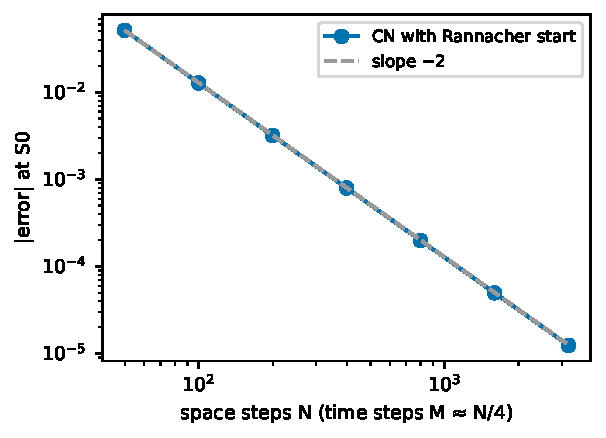
\includegraphics[width=0.55\textwidth]{cn_convergence}
\caption{Absolute error of the Crank--Nicolson price at $S_0$ for $T=1$ as both grids are refined ($M\approx N/4$); the dashed line has slope $-2$.}\label{fig:cn}
\end{figure}

\begin{table}[ht]
\centering
\caption{Separate refinement in time ($N=6400$ fixed) and in space ($M=4000$ fixed) for $T=1$: absolute price error at $S_0$ and observed order $\log_2(e_{k-1}/e_k)$.}\label{tab:refine}
\small
\begin{tabular}{rrrcrrr}
\toprule
\multicolumn{3}{c}{time refinement} && \multicolumn{3}{c}{space refinement} \\
\cmidrule(lr){1-3}\cmidrule(lr){5-7}
$M$ & error & order && $N$ & error & order \\
\midrule
10 & $2.29\times10^{-3}$ & -- && 50 & $5.01\times10^{-2}$ & -- \\
20 & $5.36\times10^{-4}$ & 2.10 && 100 & $1.24\times10^{-2}$ & 2.01 \\
40 & $1.36\times10^{-4}$ & 1.98 && 200 & $3.10\times10^{-3}$ & 2.00 \\
80 & $3.62\times10^{-5}$ & 1.91 && 400 & $7.75\times10^{-4}$ & 2.00 \\
160 & $1.13\times10^{-5}$ & 1.68 && 800 & $1.94\times10^{-4}$ & 2.00 \\
320 & $5.10\times10^{-6}$ & 1.15 && 1600 & $4.84\times10^{-5}$ & 2.00 \\
\bottomrule
\end{tabular}
\end{table}

The remaining source of error is the truncation of the domain.
\Cref{tab:domain} varies $S_{\max}$ at fixed spacing $\Delta S=0.1$ and lists, next to the price error at $S_0$, the put value at $S_{\max}$ that the far-field condition omits.
For $T=1$ a domain of $2S_0$ is already sufficient, since the error then equals the discretisation error of about $3\times10^{-5}$, but for $T=4$ the distribution of $S_T$ is much wider and the boundary error dominates until $S_{\max}=4S_0$.
The error at $S_0$ is always much smaller than the put value at the boundary, by a factor that grows rapidly with $S_{\max}$, because the boundary error is transported inwards by the diffusion and decays with the distance from the boundary.
The choice $S_{\max}=4S_0$ is thus the smallest of the tested domains that is adequate for all four maturities.

\begin{table}[ht]
\centering
\caption{Effect of the domain truncation ($\Delta S=0.1$, $M=1000$, Rannacher start): absolute price error at $S_0$ and the put value $P(T,S_{\max})$ omitted by the far-field condition.}\label{tab:domain}
\small
\begin{tabular}{rrrcrr}
\toprule
& \multicolumn{2}{c}{$T=1$} && \multicolumn{2}{c}{$T=4$} \\
\cmidrule(lr){2-3}\cmidrule(lr){5-6}
$S_{\max}/S_0$ & error at $S_0$ & $P(T,S_{\max})$ && error at $S_0$ & $P(T,S_{\max})$ \\
\midrule
1.5 & $2.2\times10^{-2}$ & $6.8\times10^{-1}$ && $9.3\times10^{-1}$ & $3.1$ \\
2.0 & $4.1\times10^{-5}$ & $6.7\times10^{-2}$ && $9.0\times10^{-2}$ & $1.3$ \\
2.5 & $3.1\times10^{-5}$ & $6.5\times10^{-3}$ && $8.6\times10^{-3}$ & $6.1\times10^{-1}$ \\
3.0 & $3.1\times10^{-5}$ & $6.7\times10^{-4}$ && $8.9\times10^{-4}$ & $3.0\times10^{-1}$ \\
4.0 & $3.1\times10^{-5}$ & $9.4\times10^{-6}$ && $2.6\times10^{-5}$ & $8.4\times10^{-2}$ \\
6.0 & $3.1\times10^{-5}$ & $5.4\times10^{-9}$ && $1.4\times10^{-5}$ & $9.9\times10^{-3}$ \\
\bottomrule
\end{tabular}
\end{table}

\subsection{Sensitivities and the Rannacher start}\label{sec:greeks}

The price comparison does not reveal any benefit of the Rannacher start: for $T=1$ the price error is $-3.4\times10^{-5}$ with and $-2.8\times10^{-5}$ without it.
The analysis of \cref{sec:cn-stab} predicts that the difference appears in the second derivative, and \cref{fig:greeks} confirms this.
On the production grid, plain CN produces a gamma that oscillates from node to node around the strike with an amplitude of about $0.013$ (\cref{fig:greeks}a), more than half of the exact gamma of $0.024$ at the strike, whereas the gamma with the Rannacher start agrees with the exact value to $1.6\times10^{-6}$ over $[0.8K,1.2K]$.
The delta is affected in the same way but less strongly, with maximal errors of $1.2\times10^{-4}$ without and $2.0\times10^{-6}$ with the start-up.

\begin{figure}[ht]
\centering
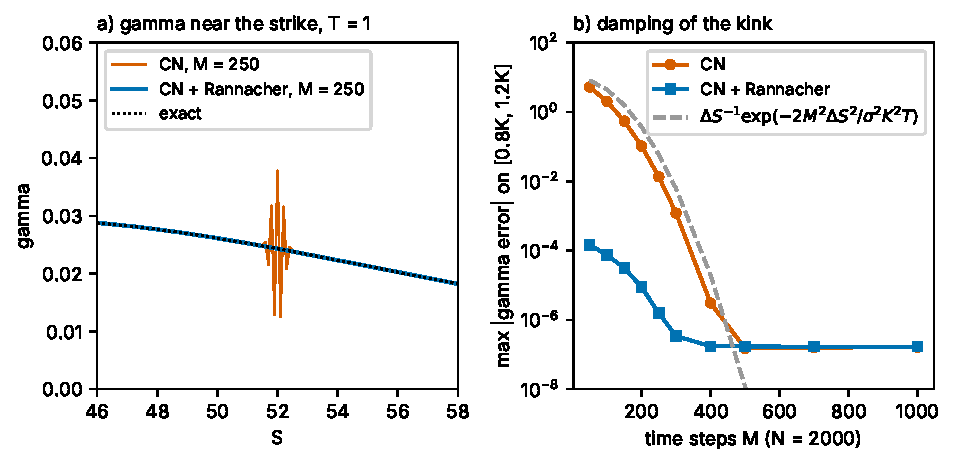
\includegraphics[width=\textwidth]{cn_greeks}
\caption{Gamma of the European call ($T=1$, $N=2000$, $\Delta S=0.1$). a) Finite-difference gamma near the strike with $M=250$ time steps, with and without the Rannacher start, and the exact gamma. b) Maximal gamma error on $[0.8K,1.2K]$ against the number of time steps, together with the frozen-coefficient estimate $\Delta S^{-1}\exp(-2M^2\Delta S^2/(\sigma^2K^2T))$ of \cref{eq:damp}.}\label{fig:greeks}
\end{figure}

\Cref{fig:greeks}b tests the damping estimate \cref{eq:damp} quantitatively.
As $M$ increases from 50 to 400 at fixed $N=2000$, the gamma error of plain CN falls from 5.2 to $3\times10^{-6}$, and the estimate, which contains no fitted constant, follows this decay over six orders of magnitude while overestimating the error by a factor of 1.6 to 6.4.
Beyond $M=500$ the kink is fully damped and both variants reach the same floor of $1.6\times10^{-7}$, which is the ordinary discretisation error of the gamma.
With the Rannacher start the gamma error is already $1.5\times10^{-4}$ at $M=50$ and decreases smoothly to the floor.
To obtain a gamma accurate to $10^{-5}$ near the strike, plain CN thus needs about 400 time steps, in agreement with the value 410 given by the bound at the end of \cref{sec:cn-stab}, while the Rannacher start achieves this accuracy with 200.
For the price at a point away from the kink the start-up procedure is immaterial, but for hedging, where the delta and gamma are the quantities of interest, it is essential.

\subsection{Accuracy of the Monte Carlo pricer}\label{sec:mc-results}

The Monte Carlo columns of \cref{tab:price} come from the MPI pricer with $10^6$ paths on 8 processes.
The plain standard errors of 0.011 to 0.028 are reduced to 0.002 to 0.004 by antithetic sampling combined with the control variate, and all 16 of the 99\% intervals contain the exact price.
The errors of the antithetic control-variate estimates are, however, all positive and lie between 1.95 and 2.07 standard errors.
This is not a sign of bias but of common random numbers: every maturity was priced with the same seed, so the four estimates are driven by the same normals and their errors are strongly correlated.
The four intervals are therefore not four independent confirmations, and the replication study below, which uses independent seeds, is the appropriate test of coverage.
As expected for a smooth one-dimensional problem, CN is far more accurate per unit of work than MC; MC becomes the method of choice for the path-dependent Asian payoff, for which no grid solver was implemented.

\subsection{Variance reduction}\label{sec:vr-results}

Having established that both methods reproduce the exact European price, we turn to the efficiency of the MC estimators.
\Cref{fig:mc} shows the root-mean-square error over 40 independent replications for sample sizes from $10^3$ to $2.56\times10^5$, and all four estimators follow the $n^{-1/2}$ rate.
\Cref{tab:vrf} lists the mean standard errors and the VRFs at $n=2.56\times10^5$ paths, together with the efficiency gain, which multiplies the VRF by the ratio of the computing times.
For the European call, antithetic sampling alone gains a factor of 1.5, the control variate 5.8 and both together 27.
For the Asian call the geometric control variate gains a factor of 511 and antithetic sampling then adds little.
Antithetic sampling also shortens the computation, since it draws half as many normals: the time for one estimate with $2.56\times10^5$ paths fell from 0.383\,s to 0.266\,s, a factor of 1.44.
With the model $t \propto (c_{\mathrm{rng}}/k + c_{\mathrm{path}})$ for $k$ paths per normal vector this factor implies that about 60\% of the cost of a path step is spent generating random variates, and it raises the efficiency gain of the combined estimator to 39 for the European and to about 750 for the Asian call.

\begin{figure}[ht]
\centering
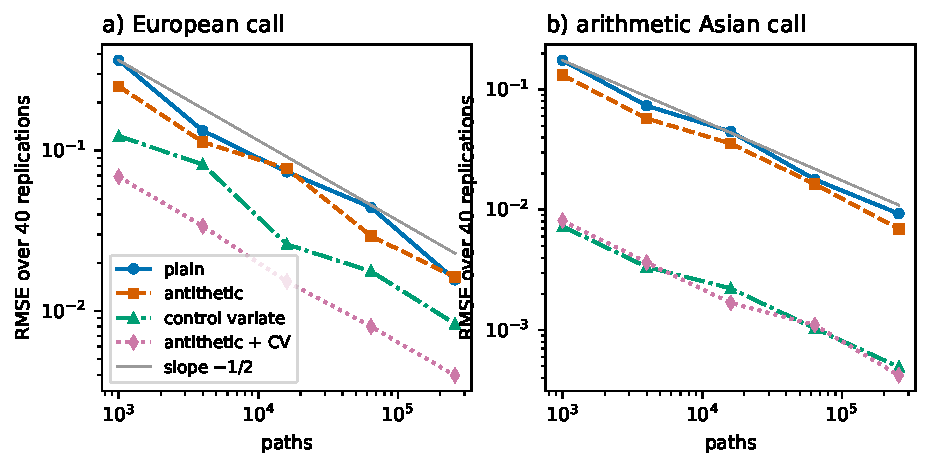
\includegraphics[width=\textwidth]{mc_convergence}
\caption{Root-mean-square error of four estimators over 40 independent replications ($T=1$, $M=252$): a) European call against the closed-form price, b) arithmetic Asian call against a reference estimate ($3.08944\pm0.00012$). The grey line has slope $-1/2$.}\label{fig:mc}
\end{figure}

\begin{table}[ht]
\centering
\caption{Mean standard error, variance-reduction factor (VRF) relative to plain MC at the same number of paths, and efficiency gain (VRF times the ratio of computing times) at $n=2.56\times10^5$ paths, 40 replications.}\label{tab:vrf}
\small
\begin{tabular}{llrrr}
\toprule
Option & Estimator & mean s.e. & VRF & efficiency gain \\
\midrule
European & plain & 0.0211 & 1.0 & 1.0 \\
 & antithetic & 0.0171 & 1.5 & 2.2 \\
 & control variate & 0.0088 & 5.8 & 5.8 \\
 & antithetic + control variate & 0.0041 & 27.0 & 38.9 \\
\midrule
Asian & plain & 0.0107 & 1.0 & 1.0 \\
 & antithetic & 0.0088 & 1.5 & 2.1 \\
 & control variate & 0.00047 & 510.6 & 510.6 \\
 & antithetic + control variate & 0.00047 & 518.9 & 747.2 \\
\bottomrule
\end{tabular}
\end{table}

The theory of \cref{sec:mc} explains these numbers quantitatively.
\Cref{tab:corr} lists the correlations measured on separate runs of $10^6$ paths and the VRFs that \cref{eq:anti,eq:cv,eq:both} predict from them.
The antithetic correlation is $-0.34$ for the European and $-0.33$ for the Asian call, negative as \cref{prop:anti} guarantees but far from $-1$, as the even--odd decomposition of \cref{sec:anti} anticipates for a convex payoff.
The correlation between the European payoff and $S_T$ is 0.909, so the control removes about four fifths of the variance, whereas the arithmetic and geometric Asian payoffs have a correlation of 0.9990, and the control removes all but a five-hundredth.
Antithetic averaging raises the payoff--control correlation of the European call from 0.909 to 0.971, which is why the two techniques combine to a factor of 27 instead of the product $1.5\times5.8 = 8.7$; for the Asian call the control already captures the nearly linear odd part of the payoff, the residual of the control-variate regression is almost an even function of the noise, and antithetic sampling, which removes only odd components, adds less than 2\%.
All six predicted factors agree with the factors observed over the 40 replications to within one percent, which confirms that the estimators behave as the asymptotic theory describes at this sample size.

\begin{table}[ht]
\centering
\caption{Correlations measured on $10^6$ paths, predicted VRFs from \cref{eq:anti,eq:cv,eq:both}, and VRFs observed over 40 replications at $2.56\times10^5$ paths (\cref{tab:vrf}). $\hat\beta$ is the control-variate coefficient without antithetic sampling.}\label{tab:corr}
\small
\begin{tabular}{lrrrrrrrrr}
\toprule
& & & & & \multicolumn{2}{c}{antithetic} & \multicolumn{2}{c}{control variate} & \multicolumn{1}{c}{both} \\
\cmidrule(lr){6-7}\cmidrule(lr){8-9}\cmidrule(lr){10-10}
Option & $\rho_a$ & $\rho_{XY}$ & $\rho_p$ & $\hat\beta$ & pred. & obs. & pred. & obs. & pred.\,/\,obs. \\
\midrule
European & $-0.338$ & 0.9095 & 0.9715 & 0.632 & 1.51 & 1.51 & 5.79 & 5.79 & 26.9\,/\,27.0 \\
Asian & $-0.326$ & 0.9990 & 0.9986 & 1.063 & 1.48 & 1.48 & 511.8 & 510.6 & 516.6\,/\,518.9 \\
\bottomrule
\end{tabular}
\end{table}

The replications also test the confidence intervals.
Across all configurations, the 99\% intervals covered the exact or reference price in 95 to 100\% of the 40 replications, which is consistent with the nominal level given the small number of replications.
To test the effect of skewness at a small sample size more precisely, we ran 1{,}000 replications of the plain European estimator with $n=2{,}000$ paths: the 99\% interval covered the exact price in 98.3\% of the cases.
The shortfall of 0.7 percentage points, about two binomial standard errors, is consistent with the Berry--Esseen bound for a payoff with skewness 2.4 and disappears at the sample sizes used for pricing.

\subsection{Exactness of the merge}\label{sec:merge-results}

To verify \cref{prop:merge} we simulated a fixed sample of $n=200{,}003$ paths, which is not divisible by any of the tested process counts, partitioned it among $p\in\{1,2,3,4,6,8,10\}$ ranks according to the rule of \cref{sec:streams}, and compared the merged estimates with the single-process estimates and with the average of the per-rank estimates.
\Cref{tab:merge} summarises the result.
The merged plain and control-variate estimates of both options differ from the single-process values by at most $1.4\times10^{-14}$ and their standard errors by at most $1.5\times10^{-16}$, which is rounding error in the summation of $2\times10^5$ terms.
Averaging per-rank estimates instead changes the plain estimates by at most $3\times10^{-5}$ standard errors, because the shares differ by one path only, but it changes the control-variate estimates by up to $0.05$ standard errors, a deviation that grows with $p$ because each rank fits its own $\hat\beta$.
These deviations are small compared with the statistical error in this balanced setting, but they make the result depend on the decomposition, which defeats the regression testing of a parallel code against its serial counterpart, and they would grow with unequal shares.
The one-pass variance formulas lose, relative to a two-pass computation, $1.1\times10^{-14}$ for the control $e^{-rT}S_T$, whose mean-to-standard-deviation ratio is the largest, and at most $4\times10^{-16}$ for the other three quantities, in line with the bound of \cref{sec:merge}.

\begin{table}[ht]
\centering
\caption{Deviation from the single-process estimates when a fixed sample of 200{,}003 paths is split among $p$ ranks: merged statistics (absolute, maximum over the four estimates) and averaged per-rank control-variate estimates (in units of the standard error).}\label{tab:merge}
\small
\begin{tabular}{rrrr}
\toprule
& merged statistics & \multicolumn{2}{c}{averaged per-rank CV estimate} \\
\cmidrule(lr){3-4}
$p$ & max.\ abs.\ deviation & European & Asian \\
\midrule
2 & $8.9\times10^{-16}$ & $-0.0004$ & $0.0003$ \\
4 & $1.4\times10^{-14}$ & $-0.0014$ & $0.0049$ \\
8 & $8.9\times10^{-16}$ & $-0.0188$ & $0.0135$ \\
10 & $4.4\times10^{-15}$ & $-0.0115$ & $0.0480$ \\
\bottomrule
\end{tabular}
\end{table}

\subsection{Parallel scaling}\label{sec:scaling}

\Cref{fig:scaling} and \cref{tab:scaling} summarise the scaling measurements as means of five repetitions with one standard deviation.
With $8\times10^6$ paths one process needs $11.7\pm0.5$\,s, which corresponds to a throughput of $1.7\times10^8$ path steps per second.
The speed-up is 1.69 on 2 processes, 2.40 on 4 and 3.49 on 8, peaks at 3.56 on 9 and falls to 3.34 on 10.
Wall times also include the \texttt{mpiexec} start-up and the Python imports, about 0.6 to 1.5\,s per job, and give lower speed-ups, for instance 2.67 on 8 processes; this overhead is the $t_0$ term of \cref{eq:perf} and would be amortised in a longer computation.

\begin{figure}[ht]
\centering
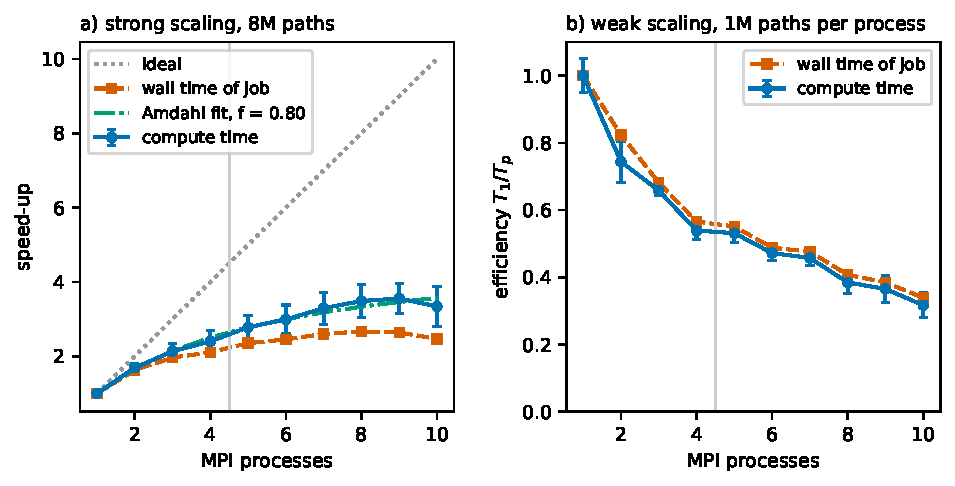
\includegraphics[width=\textwidth]{scaling}
\caption{a) Strong scaling with $8\times10^6$ paths and b) weak scaling with $10^6$ paths per process (252 steps, five repetitions, error bars one standard deviation). The grey line separates the four performance cores from the efficiency cores.}\label{fig:scaling}
\end{figure}

\begin{table}[ht]
\centering
\caption{Compute time (s, mean $\pm$ s.d. of five runs), speed-up and efficiency.}\label{tab:scaling}
\small
\begin{tabular}{rrrrrr}
\toprule
& \multicolumn{3}{c}{strong ($8\times10^6$ paths)} & \multicolumn{2}{c}{weak ($10^6$ paths per process)} \\
\cmidrule(lr){2-4}\cmidrule(lr){5-6}
processes & time & speed-up & efficiency & time & efficiency \\
\midrule
1 & 11.67 $\pm$ 0.48 & 1.00 & 1.00 & 1.48 $\pm$ 0.07 & 1.00 \\
2 & 6.91 $\pm$ 0.45 & 1.69 & 0.85 & 1.99 $\pm$ 0.16 & 0.74 \\
4 & 4.86 $\pm$ 0.61 & 2.40 & 0.60 & 2.74 $\pm$ 0.14 & 0.54 \\
6 & 3.90 $\pm$ 0.51 & 2.99 & 0.50 & 3.13 $\pm$ 0.14 & 0.47 \\
8 & 3.35 $\pm$ 0.42 & 3.49 & 0.44 & 3.84 $\pm$ 0.33 & 0.38 \\
10 & 3.49 $\pm$ 0.56 & 3.34 & 0.33 & 4.67 $\pm$ 0.55 & 0.32 \\
\bottomrule
\end{tabular}
\end{table}

The algorithmic cost of parallelisation cannot explain this loss.
Each process sends one message of 213 bytes, and the load imbalance, measured as one minus the ratio of the fastest to the slowest rank's compute time, is at most 1.7\% up to 9 processes and 4.4\% at 10.
The weak-scaling experiment isolates the cause.
There every process simulates $10^6$ paths, so that on ideal hardware the time would remain at the single-process value of 1.48\,s; instead it rises to 1.99\,s on 2 processes, 2.74\,s on 4 and 3.84\,s on 8, which corresponds to efficiencies of 0.74, 0.54 and 0.38.
In the notation of \cref{sec:perf-model}, the throughput per process thus falls to 38\% of its single-process value on 8 processes, and the aggregate throughput of the machine levels off at $5.2$ to $5.6\times10^8$ path steps per second from eight processes on, a little over three times that of a single process.

\Cref{tab:model} compares the strong-scaling speed-up with the prediction $pE_w(p)$ of \cref{eq:pred}.
The prediction reproduces the shape of the curve, including the flattening beyond four processes and the drop at ten, and it falls short of the observed speed-up by 3 to 12\%.
The systematic part of this gap is informative.
For $p=8$ the strong-scaling run and the weak-scaling run are the same job, with $10^6$ paths on each of eight ranks and the same seed, yet the former took $3.35\pm0.42$\,s and the latter $3.84\pm0.33$\,s.
The two series were run one after the other, and the difference of 15\% between identical jobs indicates that the sustained clock rate of the laptop drifted between them, presumably for thermal reasons; we did not record clock frequencies, so this attribution is an inference.
Within that uncertainty the performance model explains the strong-scaling curve completely, without any serial fraction.
Beyond four processes the work is also placed on the efficiency cores, whose lower throughput adds to the bandwidth limit and explains why the gain per additional process is smallest there.

\begin{table}[ht]
\centering
\caption{Performance model: weak-scaling efficiency $E_w(p)$, predicted strong-scaling speed-up $pE_w(p)$ from \cref{eq:pred}, observed speed-up, and aggregate throughput in the weak-scaling runs (path steps per second).}\label{tab:model}
\small
\begin{tabular}{rrrrr}
\toprule
processes & $E_w(p)$ & predicted $pE_w(p)$ & observed $S_p$ & throughput ($10^8$\,s$^{-1}$) \\
\midrule
1 & 1.00 & 1.00 & 1.00 & 1.70 \\
2 & 0.74 & 1.49 & 1.69 & 2.54 \\
4 & 0.54 & 2.16 & 2.40 & 3.67 \\
6 & 0.47 & 2.83 & 2.99 & 4.83 \\
8 & 0.38 & 3.08 & 3.49 & 5.24 \\
10 & 0.32 & 3.17 & 3.34 & 5.40 \\
\bottomrule
\end{tabular}
\end{table}

An Amdahl fit to the strong-scaling curve gives a ``parallel fraction'' of $f=0.80$, which would correspond to a serial part taking 20\% of the single-process time, or 2.3\,s.
The serial work of the program, the parameter set-up and the final merge of eleven numbers per rank, takes milliseconds, so the fitted $f$ describes the curve but does not identify any serial part of the code.
Gustafson's view \citep{gustafson1988} is the more useful one here: additional processes are best used to simulate more paths in the same time, which weak scaling achieves at 38\% efficiency on 8 processes, that is, with eight times the paths of one process in 2.6 times the time.

%% ==================================================================
\section{Discussion}\label{sec:discussion}

The experiments support three conclusions that go beyond the individual numbers.
Both pricing routes are validated against closed forms, CN through its second-order convergence in time and space and MC through confidence intervals that cover the exact price in replications with independent seeds, so the MC pricer can be trusted on the Asian option, for which no closed form exists.
The merge of additive statistics makes the parallel pricer exact in the sense of \cref{prop:merge}, so its results reproduce the single-process estimator to rounding error and do not depend on the scheduling of the ranks.
Most importantly for practice, variance reduction is a far cheaper route to accuracy than additional processes: the efficiency gain of about 750 for the Asian option corresponds to the work of 750 times as many paths, whereas the whole ten-core machine provides at most a factor of 3.6.
Since all the gains of \cref{tab:corr} are predicted by three measured correlations, a pilot run of a few thousand paths suffices to decide which technique to use for a new payoff.

The CN results carry a similar lesson for the finite-difference side.
A price comparison at a single point is a weak test of a time-stepping scheme, because the price integrates the oscillations that a non-L-stable scheme leaves behind.
The gamma exposes them, and the frozen-coefficient estimate \cref{eq:damp} predicts their size without any fitting, so that the need for the Rannacher start can be decided before computing.
The same estimate shows that the damping of plain CN depends on the product $M\Delta S$, so that for a fixed number of time steps plain CN becomes less reliable exactly when the space grid is refined for accuracy.

These conclusions are subject to the limits of the experimental set-up.
The benchmark ran on a single laptop with heterogeneous cores, so it measures the shared-memory scaling of independent processes rather than network communication; on a distributed-memory cluster each node would contribute its own memory bandwidth, the weak-scaling efficiency across nodes would be much higher, and the start-up and the gather costs would grow with the number of nodes.
The thermal drift identified in \cref{sec:scaling} also limits the precision of the timings to about 15\% between measurement series, and a cluster with fixed clock frequencies would allow a sharper test of \cref{eq:pred}.
Only the MC pricer is parallelised, since the CN solver needs about 0.04\,s at the finest tested grid.
The model is the constant-volatility Black--Scholes model, the CN solver treats only the European call, and the Asian reference value is itself an estimate with a standard error of $1.2\times10^{-4}$.

Several extensions follow naturally from these limits.
Counter-based random number generators \citep{salmon2011} would make the MC result independent of the number of processes, not only of their scheduling, by tying the random numbers to path indices.
Multilevel Monte Carlo \citep{giles2008} would lower the cost of path-dependent payoffs further by combining coarse and fine monitoring grids, and scrambled quasi-random sequences would improve on the $n^{-1/2}$ rate for smooth payoffs.
Multi-asset options are the natural setting in which MC with MPI outperforms grid methods, and they would make the communication cost on a distributed-memory cluster worth measuring.
On the finite-difference side, the same analysis applies to American options, where the early-exercise boundary introduces a second non-smoothness that moves in time.

%% ==================================================================
\section{Conclusions}\label{sec:conclusions}

We have presented an MPI Monte Carlo pricer for European and Asian options in the Black--Scholes model that merges per-process results exactly through eleven additive statistics, and we have validated it against closed-form prices and a second-order Crank--Nicolson solver.
The variance of the antithetic and control-variate estimators is determined by three correlations, and the factors predicted from them, 27 for the European and about 500 for the Asian call, agree with the observed factors to within one percent.
For the Crank--Nicolson solver, a frozen-coefficient analysis predicts the gamma error left by the payoff kink without fitted constants and shows why the Rannacher start-up is essential for the sensitivities although it barely changes the price.
The pricer reaches a $3.5\times$ speed-up on 8 processes of a ten-core laptop, and a simple performance model, in which the strong-scaling speed-up equals the number of processes times the weak-scaling efficiency, accounts for this curve without any serial fraction, attributing the loss of efficiency to shared memory bandwidth, clock limits and heterogeneous cores rather than to communication or load imbalance.

\begingroup
\small
\begin{thebibliography}{99}
\bibitem[Black and Scholes(1973)]{black1973} F.~Black and M.~Scholes. The pricing of options and corporate liabilities. \emph{Journal of Political Economy}, 81(3):637--654, 1973.
\bibitem[Crank and Nicolson(1947)]{crank1947} J.~Crank and P.~Nicolson. A practical method for numerical evaluation of solutions of partial differential equations of the heat-conduction type. \emph{Mathematical Proceedings of the Cambridge Philosophical Society}, 43(1):50--67, 1947.
\bibitem[Duffy(2006)]{duffy2006} D.~J. Duffy. \emph{Finite Difference Methods in Financial Engineering: A Partial Differential Equation Approach}. Wiley, Chichester, 2006.
\bibitem[Wilmott et~al.(1995)]{wilmott1995} P.~Wilmott, S.~Howison, and J.~Dewynne. \emph{The Mathematics of Financial Derivatives: A Student Introduction}. Cambridge University Press, Cambridge, 1995.
\bibitem[Rannacher(1984)]{rannacher1984} R.~Rannacher. Finite element solution of diffusion problems with irregular data. \emph{Numerische Mathematik}, 43(2):309--327, 1984.
\bibitem[Giles and Carter(2006)]{giles2006} M.~B. Giles and R.~Carter. Convergence analysis of Crank--Nicolson and Rannacher time-marching. \emph{Journal of Computational Finance}, 9(4):89--112, 2006.
\bibitem[Pooley et~al.(2003)]{pooley2003} D.~M. Pooley, K.~R. Vetzal, and P.~A. Forsyth. Convergence remedies for non-smooth payoffs in option pricing. \emph{Journal of Computational Finance}, 6(4):25--40, 2003.
\bibitem[Boyle(1977)]{boyle1977} P.~P. Boyle. Options: a Monte Carlo approach. \emph{Journal of Financial Economics}, 4(3):323--338, 1977.
\bibitem[Glasserman(2004)]{glasserman2004} P.~Glasserman. \emph{Monte Carlo Methods in Financial Engineering}. Springer, New York, 2004.
\bibitem[Hammersley and Handscomb(1964)]{hammersley1964} J.~M. Hammersley and D.~C. Handscomb. \emph{Monte Carlo Methods}. Methuen, London, 1964.
\bibitem[Lavenberg and Welch(1981)]{lavenberg1981} S.~S. Lavenberg and P.~D. Welch. A perspective on the use of control variables to increase the efficiency of Monte Carlo simulations. \emph{Management Science}, 27(3):322--335, 1981.
\bibitem[Kemna and Vorst(1990)]{kemna1990} A.~G.~Z. Kemna and A.~C.~F. Vorst. A pricing method for options based on average asset values. \emph{Journal of Banking \& Finance}, 14(1):113--129, 1990.
\bibitem[Glynn and Whitt(1992)]{glynn1992} P.~W. Glynn and W.~Whitt. The asymptotic efficiency of simulation estimators. \emph{Operations Research}, 40(3):505--520, 1992.
\bibitem[Esary et~al.(1967)]{esary1967} J.~D. Esary, F.~Proschan, and D.~W. Walkup. Association of random variables, with applications. \emph{Annals of Mathematical Statistics}, 38(5):1466--1474, 1967.
\bibitem[Chan et~al.(1983)]{chan1983} T.~F. Chan, G.~H. Golub, and R.~J. LeVeque. Algorithms for computing the sample variance: analysis and recommendations. \emph{The American Statistician}, 37(3):242--247, 1983.
\bibitem[O'Neill(2014)]{oneill2014} M.~E. O'Neill. PCG: a family of simple fast space-efficient statistically good algorithms for random number generation. Technical Report HMC-CS-2014-0905, Harvey Mudd College, 2014.
\bibitem[Salmon et~al.(2011)]{salmon2011} J.~K. Salmon, M.~A. Moraes, R.~O. Dror, and D.~E. Shaw. Parallel random numbers: as easy as 1, 2, 3. In \emph{Proceedings of the International Conference for High Performance Computing, Networking, Storage and Analysis (SC11)}, 2011.
\bibitem[L'Ecuyer et~al.(2017)]{lecuyer2017} P.~L'Ecuyer, D.~Munger, B.~Oreshkin, and R.~Simard. Random numbers for parallel computers: requirements and methods, with emphasis on GPUs. \emph{Mathematics and Computers in Simulation}, 135:3--17, 2017.
\bibitem[Dalcin et~al.(2005)]{dalcin2005} L.~Dalcin, R.~Paz, and M.~Storti. MPI for Python. \emph{Journal of Parallel and Distributed Computing}, 65(9):1108--1115, 2005.
\bibitem[Hockney(1994)]{hockney1994} R.~W. Hockney. The communication challenge for MPP: Intel Paragon and Meiko CS-2. \emph{Parallel Computing}, 20(3):389--398, 1994.
\bibitem[Thakur et~al.(2005)]{thakur2005} R.~Thakur, R.~Rabenseifner, and W.~Gropp. Optimization of collective communication operations in MPICH. \emph{International Journal of High Performance Computing Applications}, 19(1):49--66, 2005.
\bibitem[Williams et~al.(2009)]{williams2009} S.~Williams, A.~Waterman, and D.~Patterson. Roofline: an insightful visual performance model for multicore architectures. \emph{Communications of the ACM}, 52(4):65--76, 2009.
\bibitem[Amdahl(1967)]{amdahl1967} G.~M. Amdahl. Validity of the single processor approach to achieving large scale computing capabilities. In \emph{Proceedings of the AFIPS Spring Joint Computer Conference}, pages 483--485, 1967.
\bibitem[Gustafson(1988)]{gustafson1988} J.~L. Gustafson. Reevaluating Amdahl's law. \emph{Communications of the ACM}, 31(5):532--533, 1988.
\bibitem[Giles(2008)]{giles2008} M.~B. Giles. Multilevel Monte Carlo path simulation. \emph{Operations Research}, 56(3):607--617, 2008.
\end{thebibliography}
\endgroup

\end{document}
